\section{RESULTS AND DISCUSSION}

We report the pipeline in the order it runs, then turn the verifier on itself. Pass counts are fractions; the intervals that belong to them appear with the acceptance-criterion results.

\subsection{Face-Level Machining Feature Recognition}

The three-layer message-passing network reaches 0.9660 accuracy and 0.9042 mean intersection over union on the MFCAD++ test split (Figure~\ref{fig:2}). Removing edge features yields 0.6969 and 0.4462 on the same held-out test split, supporting their usefulness in this recognition model. A decision tree records 0.9075 and 0.7198 on a different validation split; these historical values are reported for context, not as a matched test-set comparison or evidence of superiority. Recognition is an upstream component, not the principal contribution or a demonstration of foundation-model multimodal learning.

\begin{figure}[htbp]
  \centering
  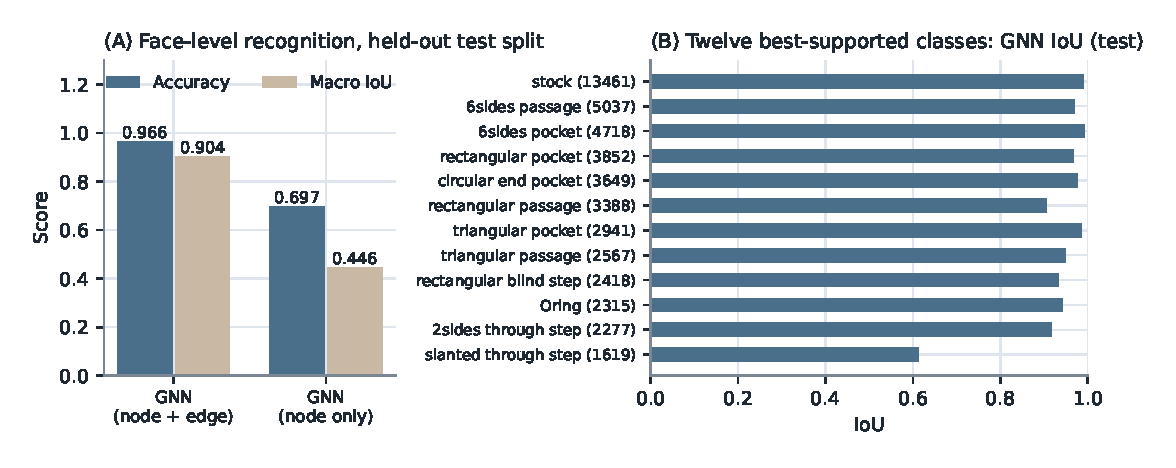
\includegraphics[width=\textwidth]{fig2.pdf}
  \caption{Face-level machining feature recognition. (A) Graph-network and node-only results on the same held-out test split. (B) Per-class intersection over union for the twelve best-supported classes under the full model, with test face counts in parentheses.}
  \label{fig:2}
\end{figure}

\subsection{Three Routes Compared on the Anchor Parts}

Table~\ref{tab:1} and Figure~\ref{fig:3} compare three ways of producing a program for the same ten parts, the same stock and the same cutters. A conventional face-milling route built from FreeCAD Path operators passes 2 of 10. A bounding-box plan produced by our own earlier generator passes 2 of 10. The region-masked generator passes 10 of 10, with zero total gouging and a worst mean deviation of 0.206 mm.

\begin{table}[htbp]\small
\caption{Three toolpath routes on the ten anchor parts. Gouge volume is summed across parts; mean absolute deviation is reported for the worst part. Passes use Equation~\ref{eq:accept}.}
\centering
\begin{tabular}{lccc}
\toprule
Route & Total gouge (mm$^3$) & Worst mean deviation (mm) & Dual-line pass \\
\midrule
FreeCAD Path operators & 215,126.7 & 12.225 & 2/10 \\
Bounding-box plan & 196,726.7 & 12.118 & 2/10 \\
Region-masked plan & 0.0 & 0.206 & 10/10 \\
\bottomrule
\end{tabular}
\label{tab:1}
\end{table}

\begin{figure}[htbp]
  \centering
  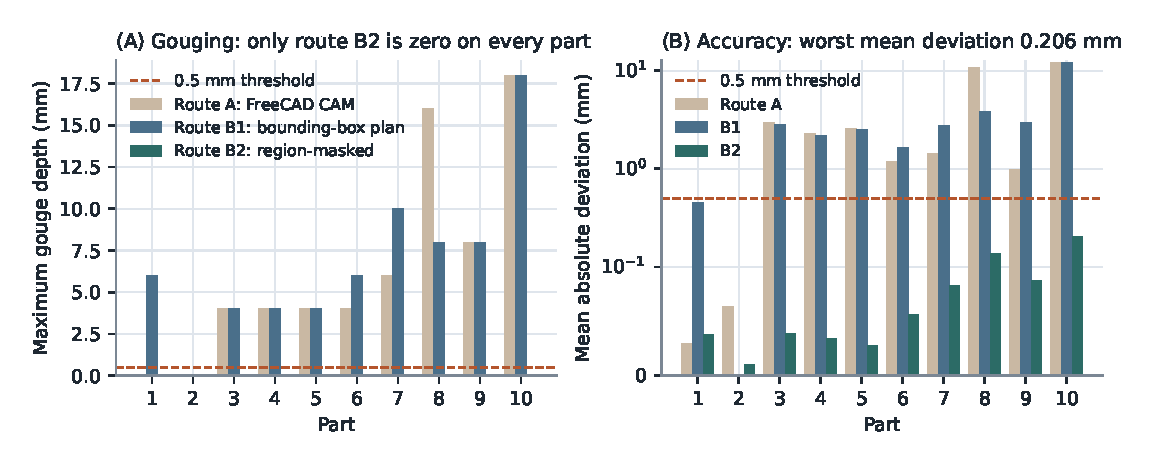
\includegraphics[width=\textwidth]{fig3.pdf}
  \caption{Three toolpath routes on the ten anchor parts. (A) Maximum gouge depth and (B) mean absolute deviation; dashed lines mark the 0.5 mm threshold. Gouging under the region-masked route is identically zero within the discrete representation.}
  \label{fig:3}
\end{figure}

The failure of the conventional route is a semantic one, and we report it as a negative result. Its face-milling operator is defined to machine flat to a given height; when several disconnected regions share that height, the toolpath degenerates to the bounding box of all of them. Four boundary configurations were tried and none constrained the traversal. This says that a general-purpose facing operator does not match layer-by-layer machining on multi-level pockets. It does not say that the underlying computer-aided manufacturing package is incapable of machining these parts with a full process setup.

Switching off the radius inflation in Equation~\ref{eq:mask}, with everything else unchanged, takes the dual-line result from 10/10 to 0/10 and produces a worst gouge of 18.000 mm. Without inflation, a tool centre can approach a step while the cutter overlaps the higher plateau; the resulting vertical gouge depends on the local height difference, not on adding a horizontal cutter radius to that height. The internal zero-gouging result does not come from knowing which regions to keep. It comes from dilating those regions by the cutter radius before placing any tool centre.

\subsection{Failure of a Single Maximum-Deviation Criterion}

A single $\max|S-P|$ does not distinguish excess removal from residual stock (Figure~\ref{fig:4}). Our dual-line criterion makes that distinction, at the cost of accepting some large local residuals; this choice is not a replacement for a part-specific dimensional tolerance. Four observations support Equation~\ref{eq:accept}. First, the worst 10 mm deviation under the region-masked route is entirely residual: maximum gouge depth is 0.000 mm on all ten parts, and every column above threshold has material higher than the target, which a finishing pass can remove. Second, the same toolpath's maximum deviation is an artefact of resolution: coarsening the grid from 0.5 to 1.0 mm changes the worst deviation on parts 1, 8 and 10 from 6, 8 and 10 mm to 0, 0 and 0 mm, simply because the narrow columns disappear. Third, on the worst part, 2.844 percent of columns exceed 0.5 mm and all of them lie within one cell of a step boundary; they form a single connected cluster. This is a cutter that cannot reach, not a path that wandered. Fourth, adding a 0.75 mm finishing cutter drives mean deviation to zero, but the program grows from 10,439 to 28,245 lines. This is a sensitivity example under the discrete model, not a proof of attainable physical accuracy or a proposed production process.

\begin{figure}[htbp]
  \centering
  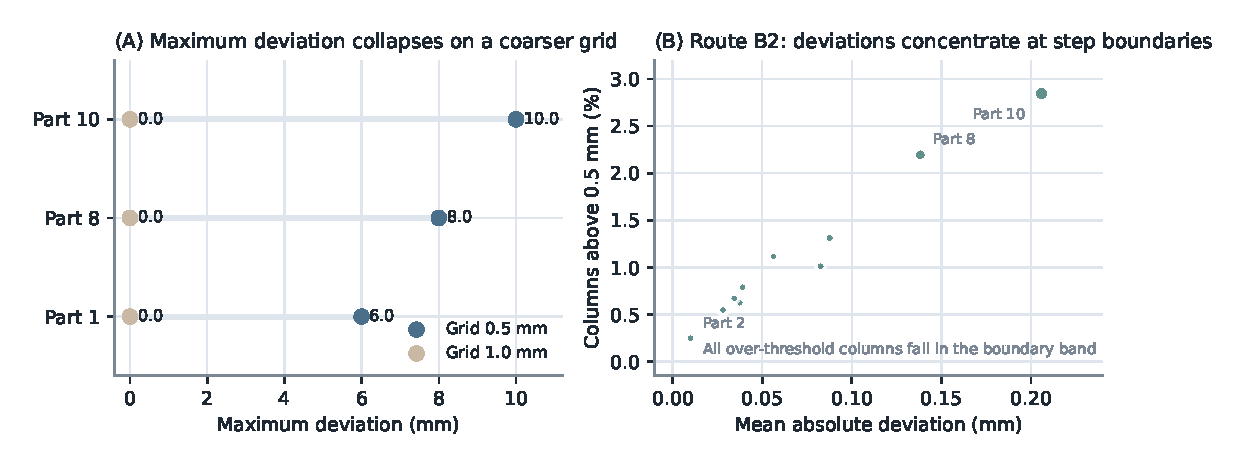
\includegraphics[width=\textwidth]{fig4.pdf}
  \caption{Behaviour of the acceptance criterion. (A) Maximum deviation of an identical toolpath under two grid resolutions; the coarser grid collapses the maximum to zero. (B) Fraction of columns above threshold and mean deviation for the region-masked route; marker area shows residual volume.}
  \label{fig:4}
\end{figure}

\begin{table}[htbp]\small
\caption{Wilson 95\% score intervals for every pass count cited in the main claims. Counts are reported as $k/n$ rather than percentages; the Wald interval degenerates at proportions of 0 and 1.}
\centering
\begin{tabular}{lccc}
\toprule
Result & $k/n$ & Point estimate & Wilson 95\% interval \\
\midrule
Region-masked dual-line pass & 10/10 & 1.000 & [0.7225, 1.0000] \\
FreeCAD operator route & 2/10 & 0.200 & [0.0567, 0.5098] \\
No-inflation baseline & 0/10 & 0.000 & [0.0000, 0.2775] \\
End-to-end without / with repair & 2/20, 20/20 & 0.100, 1.000 & [0.0279, 0.3010], [0.8389, 1.0000] \\
Third-party generated toolpath & 9/10 & 0.900 & [0.5958, 0.9821] \\
External set dual-line pass & 130/130 & 1.000 & [0.9713, 1.0000] \\
\bottomrule
\end{tabular}
\label{tab:2}
\end{table}

Table~\ref{tab:2} gives nominal score intervals under an independent Bernoulli sampling model. The anchor set is curated, the external set is geometrically filtered, and the twenty orchestration tasks reuse ten designs. These intervals therefore do not establish industrial-population reliability, and the two stock variants must not be interpreted as twenty independent designs. The external set expands geometric coverage; it does not convert the internal criterion into an externally validated safety guarantee.

\subsection{Orchestration and Bounded Repair}

Twenty tasks were formed from the ten parts at two stock allowances (1.0 and 2.5 mm), with part family derived from the number of target height layers (Figure~\ref{fig:5}). With repair disabled, 2 of 20 pass. With repair enabled and cold memory, 20 of 20 pass at a mean 0.90 repair rounds. With warm memory, 20 of 20 pass at 0.15 rounds, and 17 of 20 are accepted on the first attempt rather than 2. Split by family, the unrepaired bounding-box plan passes 0.500 of parts with at most two layers and 0.000 of parts with three or more; the more layers there are, the less a single bounding box resembles the part.

\begin{figure}[htbp]
  \centering
  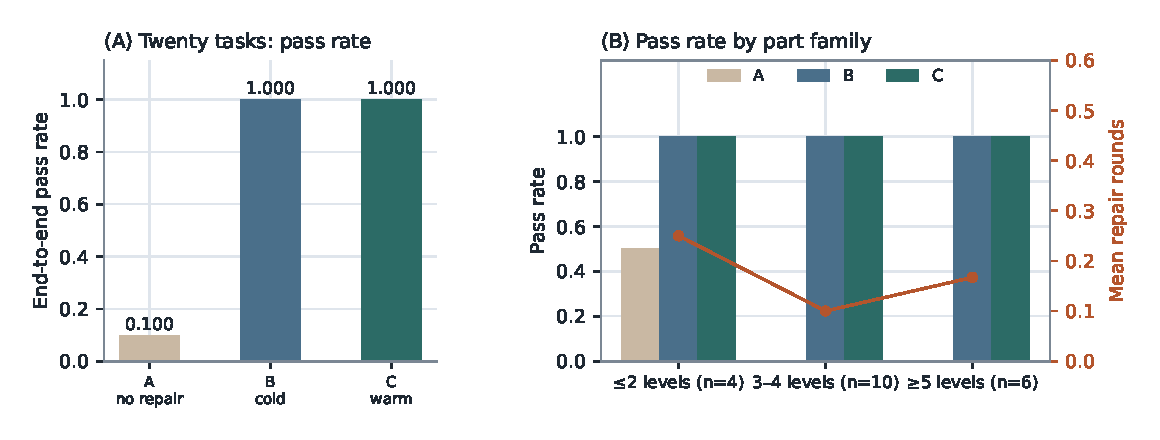
\includegraphics[width=\textwidth]{fig5.pdf}
  \caption{Orchestration ablation over twenty tasks. (A) End-to-end pass rate with repair disabled, with cold memory and with warm memory. (B) Pass rate by part family; the line shows mean repair rounds for the warm-start group.}
  \label{fig:5}
\end{figure}

The 20/20 describes recovery within a constructed suite, not general agent capability. The final repair option is a region-masked plan already known to pass these anchor designs; zero internal gouging alone would not guarantee the residual-error condition on another design. The 2/20 without repair and the drop from 0.90 to 0.15 rounds describe the cost of starting from a poor plan and reusing remedies. The six roles were deterministic strategies at this stage. The twenty tasks reuse ten geometries, and warm memory is evaluated within this constructed sequence, not on a held-out family split.

\subsection{Fifteen Models at the Decision Points}

Two semantic choices were handed to Qwen3-8B: planning strategy (bounding box or height map) and repair action (switch or escalate). Geometry and verification stayed deterministic. Table~\ref{tab:3} collects the action-space comparison that frames the paper.

\begin{table}[htbp]\small
\caption{Archived work-order comparison for Qwen3-8B. Exports are not semantic successes. Agreement means removed-volume IoU $\geq0.9$ against the original contract-generated reference. All-task means include failed exports as zero. These references are audited separately below.}
\centering
\begin{tabular}{llccc}
\toprule
Interface & Set & Exports & Agreement & All-task IoU \\
\midrule
Contract & Easy & 20/20 & 20/20 & 0.985 \\
Script & Easy & 19/20 & 2/20 & 0.165 \\
Contract, run 1 & Hard & 30/30 & 22/30 & 0.789 \\
Contract, run 2 & Hard & 30/30 & 22/30 & 0.769 \\
Script, run 1 & Hard & 26/30 & 2/30 & 0.099 \\
\bottomrule
\end{tabular}
\label{tab:3}
\end{table}

Under a neutral prompt the model chose the conservative height-map strategy 20/20 times and ignored cycle time. Rewriting one sentence to state that every hundred program lines cost about thirty seconds flipped all twenty decisions to the aggressive strategy, including parts with ten layers that necessarily gouged. No conditional behaviour by layer count appeared; the model followed the most salient instruction, not the geometry. Eighteen of twenty runs in that group gouged on the first attempt, up to 18 mm, and were rescued only by bounded repair. The verifier, not the model, decided whether the repaired outcome was acceptable. Choosing the masked strategy was not free: the mean of twenty per-task program-length ratios is 11.37. Total line counts are 59,788 versus 4,682; the mean ratio is not the ratio of these totals. The cycle-time statement was a prompt heuristic, not a measured machining-time model. Archived calls used about 350 tokens and 0.15--0.25 s per call.

Structured errors did not improve model repair. Three feedback conditions -- structured fields, prose, and no numeric values -- produced identical pass rates, identical repair-round distributions and identical action choices, while the structured version spent 79 percent more prompt tokens. With only two repair options and an obvious answer, the model had no use for the numbers. We therefore make no claim that structured errors improve language-model repair; we claim they let the \emph{program} locate the offending operation, which is what the deterministic repairer consumes.

The original easy-set archive records exports on 20/20 contract tasks and 19/20 script tasks. Its conditional mean removed-volume IoUs are 0.985 and 0.174; counting the failed script as zero changes the latter all-task mean to 0.165. These scores are agreement with the archived reference, not independent proof of correctly following each order. Thirteen contract tasks contain recorded execution errors, with 19 error entries in total, even though all twenty meet the original IoU threshold. The executor continues after a rejected call, and the original reference uses that same executor. Agreement can therefore reward a feature omitted from both outputs.

The independent reconstruction is only partly complete. For the contract route it rescores all twenty tasks against a full-precision target: mean removed-volume IoU is 0.7526, and 9 of 20 reach 0.9. The gap from the archived 0.985 is expected: the reconstructed target includes cutters that the gateway had rejected, so it credits material the archived reference also omitted. The prompt-visible target gives 0.7871 over the 19 tasks that can be scored; NL07 remains unresolved because its rounded reference produces Boolean cells that fail the volume identities. The script route is bounded rather than estimated: NL03 shares the stock's outer shell, so OCC returns the stock unchanged from \texttt{stock.cut(output)} while \texttt{output.cut(stock)} returns the output, and no comparison satisfies the volume identities. With failed exports counted as zero and the unresolved tasks left null, the script mean lies between 0.1788 and 0.2288 against the full-precision target and between 0.1811 and 0.2811 against the visible target. These are bounds, not point estimates. The reconstruction uses the same Open CASCADE kernel; it validates reference-construction logic, not cross-kernel agreement.

Table~\ref{tab:3} also reports the retained thirty-item hard-set runs rather than the earlier eight-item pilot, whose complete per-item report is no longer available. Those hard-set scores remain conditional on the original reference construction. Removed-volume scoring is still important: in a retained corner-placement example, whole-solid IoU is 0.933 while removed-volume IoU is zero. It avoids dilution by unchanged stock, but cannot correct a defective reference.

The fifteen-model contract study uses thirty orders and a common interface template. Fourteen models export 30/30 outputs; Llama-3.1-8B exports 29/30 because one response fails JSON parsing. The recorded legality metric is 1.000 over emitted calls for every available model, but it counts known tool names and required-argument presence before execution. A failed response contributes no calls to that denominator, and rejected commits need not reduce it. It therefore establishes neither perfect syntax across responses nor semantic correctness. Conditional removed-volume IoU against the archived reference spans 0.462--1.000, with the best local mean 0.842; six cloud models meet the archived geometric criterion on all thirty orders. One additional endpoint returns HTTP 400 for all thirty requests and is reported separately as unavailable, not as a model-capability failure. Parameter counts do not isolate a scale effect: model families, training and quantisation differ, and cloud counts are undisclosed.

One item exposed an ambiguity in the task set. The original wording specified two pockets symmetric about a line without stating their distance from it; eight of nine models produced other defensible layouts. Adding the missing distances and rerunning only that item took the ten cloud models from 1 correct to 10/10 at intersection over union 1.0, while all five local models still failed. A benchmark has to be shown unambiguous before it can be used to rank models, and this episode also sets a boundary on the contract: all fifteen models had perfect legality, and not one asked for the missing distance.

A second, harder set of twenty orders targeted only the weaknesses that data had exposed -- compound depths, implicit constraints and negation chains -- with every item made uniquely solvable. It widened the cloud--local gap from 0.158 to 0.239 and cut the number of error-free cloud models from six to three, but did not fully separate the frontier models. Where errors remain is more informative than the score: cloud models fail almost exclusively on jointly satisfying several spatial constraints, and barely fail at arithmetic; local models show the opposite pattern. Adding a genuinely different geometry did not add difficulty. A sloping-bottom pocket, implemented with a new contract operation, was solved 6/6 by nine of ten cloud models and by three of five local models, including the two smallest local models that scored worst elsewhere. The parameter names are literal and the order states the numbers directly. Difficulty came from how much had to be inferred, not from how complex the feature was. The extension cost thirty lines in the geometry worker, one schema entry and one precondition; the height field, the removal simulator and the evaluation pipeline were untouched.

When requirements were deliberately incomplete, the correct behaviour was to ask. Five under-specified orders were given two permitted outputs, a set of calls or a clarification. Cloud models hit 3.1 of 4 strong ambiguities and local models 0.8 of 4; human scoring of clarification quality on a 0--2 scale gave cloud models 6.8 of 8 against 0.8 of 8 locally. Two observations complicate ranking by a single score. A cloud model with 0.973 on the hard set hit only 1 of 4 clarifications, while a local model with 0.412 hit 2 of 4 -- the best local result. A model that never asks will confidently machine an ambiguous drawing, so a ranking built only on intersection over union is not a ranking of shop-floor safety. We also learned that ``depth 1'' was read as 1 mm by all fifteen models: an engineering default is not an ambiguity, and a test that treats it as one records correct behaviour as an error.

Bounded multi-round repair solved 9 of 10 harder orders within two rounds, but two feedback forms again gave identical per-task outcomes and differed only in prompt tokens. A controlled probe on the one item that resisted repair -- ``upper-left corner'' read as centre -- fixed the wrong plan and varied only the feedback, three times each. Vague feedback succeeded 0/3; structured feedback naming leftover material succeeded 0/3; structured feedback that supplied the correct coordinates succeeded 3/3. This probe does not establish that feedback can never repair misunderstanding; it shows failure under the evaluated model, item and feedback budgets. Our deterministic repairer works because it receives operation identifiers and face identifiers, not a sentence saying something is wrong.

Asked to write machine instructions directly, with the stock, feature extents, target heights and allowed code set all supplied, the model passed 0/10. Eight of the ten programs were whitelist-legal, yet none was geometrically correct; the deepest cut reached 48 mm. Free-form modelling scripts ran on 3 of 5 parts and met a 5 percent volume tolerance on 1 of 5, failing for semantic reasons such as constructing a compound instead of a Boolean difference. The problem is not whether the model can write code. It is whether the code knows that material has to be removed.

An offline diagnostic raises the endpoints of the ten archived programs to the nearest target-column height, without adding passes or changing horizontal coordinates. It still gives 0/10: mean worst gouge falls from 10.596 to 4.996 mm, while mean residual volume rises from 25,503 to 25,623 mm$^3$. This operation does not compute clearance for the full cutter footprint or the interior of every segment, and is therefore neither a safe projection nor an upper bound on repair. It demonstrates only that this particular endpoint-lifting heuristic does not rescue the programs. An iterative model or planner allowed to add coverage was not evaluated.

These results motivate restricting what the deployed model may emit while retaining independent checks on the resulting geometry. Free-form programs are not intrinsically unjudgeable: they can be executed in an appropriate sandbox and checked geometrically. The present results concern the tested implementations and prompts, not an impossibility of repairing free-form outputs.

\subsection{Auditing the Verifier Itself}

Ten anchor parts and a self-written simulator invite two questions, so we addressed both with code that does not share our algorithms (Figure~\ref{fig:6}, Table~\ref{tab:4}). The external set of 130 parts passes the same dual-line criterion 130/130, with worst gouge 0.000 mm and worst mean deviation 0.306 mm; every height-layer group from 3 to 10 passes fully.

\begin{table}[htbp]\small
\caption{Third-party audit of the acceptance criterion. Percentages are fractions of sampled tool-centre positions judged by continuous cutter--triangle intersection.}
\centering
\begin{tabular}{lcc}
\toprule
Measure & Ten anchor parts & 130 external parts \\
\midrule
Third-party gouge under region-masked plan & 0.76\% (2,822/371,230) & 3.275\% (316,398/9,660,095) \\
Third-party gouge without inflation & 10.59\% (43,260/408,646) & 14.468\% (1,571,946/10,865,228) \\
Our dual-line pass, region-masked & 10/10 & 130/130 \\
With half-cell guard, gouge count & 41 & 5,167 \\
With half-cell guard, dual-line pass & 9/10 & 107/130 \\
With half-cell guard, residual volume & 3.4$\times$ & 4.42$\times$ \\
Parts with any flag, plain / guarded & -- & 128/130, 19/130 \\
Parts with deep flag, plain / guarded & -- & 94/130, 8/130 \\
Worst cutter depth (mm), plain / guarded & -- & 71.104, 42.288 \\
\bottomrule
\end{tabular}
\label{tab:4}
\end{table}

CAMotics simulates the same programs, stock and cutters and reports the remaining workpiece volume; across ten parts the mean relative difference from our remaining-volume figure is 1.15 percent (maximum 3.22, 95th percentile 2.90). Because the stock is identical, this is also an aggregate statement about removed volume, but it does not establish pointwise agreement or equal acceptance decisions; the difference grows with the number of layers because step boundaries get longer. OpenCAMLib answers a question CAMotics cannot: whether an individual tool-centre position contacts material in continuous geometry. Its point-cutter height field agrees with our rasterisation on at least 99.828 percent of 256,000 columns at 1.0000 coverage intersection over union, with 120 columns differing at curved step edges. It rejects the no-inflation baseline at 10.59 percent of positions while flagging only 0.76 percent under the region-masked plan, and it produces none of those flags for toolpaths it generates itself. Our criterion accepts 9/10 of those third-party toolpaths; part 10 fails the accuracy line at 0.538 mm with genuine residual material and zero gouging. A verifier that rejects a bad route and accepts an independently produced good one is not simply rubber-stamping its own generator.

An independent geometry chain speaks to the input mesh. Tessellating the STEP files through FreeCAD into binary STL and reading them with OpenCAMLib, bypassing our JSON cache, reproduces the height field to at least 99.984 percent column-wise. Four purely planar parts differ by 0.0000 mm; the six parts with curved faces differ on 15 columns total (at most 0.06 percent) by one layer depth, because two tessellators cut arcs differently. Gouge counts change from 2,822/43,260 to 2,826/43,262, under 0.15 percent. STEP parsing still uses Open CASCADE, so this is an independent triangulation, serialisation and geometry-reading path, not a second boundary-representation kernel.

The audit also found a blind spot that we would not otherwise have seen, and we report it rather than smoothing it away. Radius inflation measures distance from column centre to column centre, whereas continuous geometry measures from column centre to step edge; near an arc the discrete mask can under-cover by half a cell, and the generator and verifier share the disc that hides it. Three observations identify this as a resolution artefact. Refining the grid on one part from 0.5 through 0.25 to 0.125 mm reduces the third-party gouge rate monotonically from 1.332 to 0.432 to 0.143 percent. Adding a half-cell guard to the inflation radius cuts gouge positions from 2,822 to 41. But the guard has a real cost: residual volume rises from 4,606 to 15,886 mm$^3$, and the dual-line result falls from 10/10 to 9/10. Thus this tested guard does not achieve both objectives on the evaluated set. This is not an impossibility result for other paths, cutters or continuous-offset constructions.

The external set exposes a more serious disagreement. Grid coverage averages 96.849 percent and falls to 77.465 percent. A finite-radius cutter may touch a neighbouring plateau even when its centre lies in a column omitted from the target mask; that interaction is absent from the internal check. Column-centre dilation also misses contact at slanted boundaries. The finite-cutter oracle flags 316,398 sampled positions, including 77,363 deeper than 0.5 mm, with a maximum predicted depth of 71.104 mm. These are not uniformly shallow violations.

A revision audit aggregates by part rather than treating millions of correlated path samples as independent trials. The unguarded plan has at least one flag on 128/130 parts and a violation deeper than 0.5 mm on 94/130 (Wilson 95\% CI 0.64--0.79). With a half-cell guard those counts fall to 19/130 and 8/130 (0.03--0.12), but the maximum finite-cutter depth remains 42.288 mm. Equal-weight mean per-part flag rates are 3.1973 percent and 0.0384 percent, respectively; pooled-point rates are 3.2753 percent and 0.0558 percent. The guard never moves a part from non-violating to violating: 86 parts improve, none worsen, eight remain above the line and 36 stay below it (exact McNemar $p<10^{-25}$). The count is not a knife-edge threshold effect: it is 102/130 at 0.25 mm, 94/130 from 0.5 to 5 mm, 87/130 at 10 mm and 49/130 at 20 mm; the guarded count is 13/130 at 0.25 mm, 8/130 at 0.5 mm and 6/130 from 0.75 mm upward. Violations concentrate where mask coverage is low: 34/36 parts below 96\% coverage exceed 0.5 mm, against 28/32 at 96--99\% and 32/62 at 99\% or above (Spearman $\rho=-0.42$ for coverage against the binary violation indicator). This association is consistent with the coverage mechanism; it does not establish coverage as the only cause. The guard reduces exposure, but does not eliminate the external safety failures.

Point-probe sensitivity is a different measurement. Shrinking the geometry probe from Ø0.02 to Ø0.002 mm reduces discrepant columns from 199 to 2; a Ø0.0002 mm probe leaves one. This explains sensitivity in pointwise mesh reconstruction, not the finite-radius toolpath violations. The value 71.104 mm occurs in both fields of the archive. It cannot be dismissed as a point-probe artifact in the toolpath audit, which uses operation-specific cutters. All these depths are predictions on a tessellated model, not measurements of physical cutting.

Accordingly, zero gouging is restricted to the internal single-valued height-field representation and shared discrete disc. Passing that criterion does not establish continuous-mesh safety: the external oracle disagrees on most unguarded parts. The disagreement is a measured limitation of the proposed generator--verifier pair, not a safety issue resolved merely by disclosing it.

\begin{figure}[htbp]
  \centering
  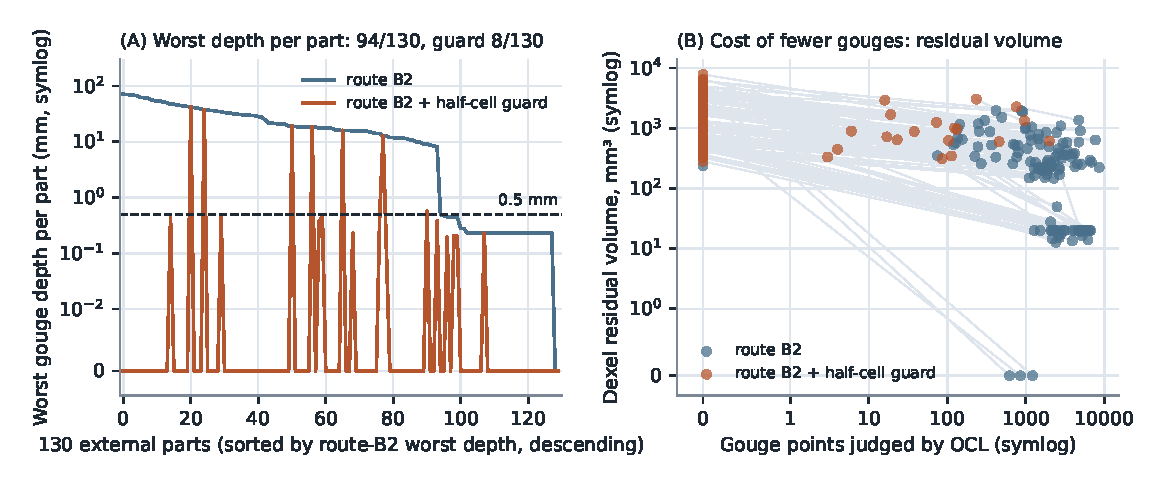
\includegraphics[width=\textwidth]{fig6.pdf}
  \caption{Third-party criterion over 130 external parts with operation-specific cutters. (A) Worst predicted gouge depth per part for the plain mask and with the half-cell guard, sorted by the plain-mask depth; the dashed line is 0.5 mm. (B) Per-part shift from the plain to the guarded mask: fewer judged gouge points, more residual volume. Both axes use symlog scaling so that exact zeros remain visible rather than being replaced by a display floor.}
  \label{fig:6}
\end{figure}

\subsection{Verifier Self-Check and Human Agreement}

On the anchor set the verifier processes 65 operations, 2,271 program lines and 1,797 parsed segments, with whitelist checks passing 10/10. Injected gouging, residual material and interference are each detected 10/10; a clean program raises no false interference alarm. Nine error objects carry operation identifiers, face identifiers and per-operation attribution, and six design-for-manufacture warnings (fillet radii below cutter radius, and similar) are reported without being used to judge acceptance.

Three computer numerical control programmers answered 30 binary questions each and agreed with the verifier at $\kappa=1.000$. We downgrade this to a sanity check. The visualisation legend fixed red to gouging and the question was exactly ``is there gouging?'', so a trivial classifier that counts red pixels also scores 1.0000. The experiment shows only that the alarms and the pictures do not contradict each other; it is not evidence of independent human judgement. A construct-validity study would need an information channel decoupled from the simulator output, such as giving readers the toolpath and the drawing without the heat map.
